% csposter.tex : example usage of the CS poster template file
% version : 18/09/17
% IMPORTANT:
% Several paper sizes are available, a0paper is probably what you're looking for.
% If you need another paper size, be sure to use the fontscale option to scale the default font size to something 
% reasonable (smaller scale means bigger font), e.g. \documentclass[a4paper,fontscale=1.4]{csposter}
% If you want a landscape format, use the extra "landscape" option in combination with another paper format.
% For posters that need to fit the departmental frames, use \documentclass[a1paper,fontscale=0.5]{csposter}.
% example options:
\documentclass[a0paper]{csposter}
%\documentclass[a0paper,landscape]{csposter}
%\documentclass[a1paper,fontscale=0.5]{csposter}
%\documentclass[a1paper,fontscale=0.5,landscape]{csposter}
%\documentclass[a4paper,fontscale=1.4]{csposter}
%\documentclass[a4paper,landscape,fontscale=1.4]{csposter}

% load custom commands, macro's etc.
% !TEX root = csposter.tex
%%
%% This is `cspostershared.tex', a header file for `csposter.tex' that contains the specification of
%%   - packages
%%   - custom commands
%%   - user defined macro's
%% Extend this file with your own packages and/or macro's

% the KU Leuven Handbook of Style specifies Helvetica Neue as the standard font
\DeclareRobustCommand{\helvetica}{%
	\fontencoding{\encodingdefault}%
	\fontseries{m}
	\fontshape{n}
	\fontfamily{phv}
	\fontsize{9}{12}
	\selectfont
}

%%%%%%%%%%%%%%%%%%%%%%%%%%%%%%%%%%%%%%%%%%%%%%%%%%%%%
% PACKAGES
%%%%%%%%%%%%%%%%%%%%%%%%%%%%%%%%%%%%%%%%%%%%%%%%%%%%%

% do not remove any of the following packages
\usepackage[T1]{fontenc}
\usepackage{amssymb, amsmath, mathtools}
	\mathtoolsset{showonlyrefs}
\usepackage{geometry}
\usepackage{color}
\usepackage{graphicx}
\usepackage{ pgfplots}
	\pgfplotsset{compat=newest}
	\newlength\figureheight
	\newlength\figurewidth
\usepackage{tikz}
	\usetikzlibrary{backgrounds}
	\usetikzlibrary{calc,shapes,backgrounds,fit,arrows,positioning,decorations.pathmorphing}
	%\usetikzlibrary{external}
	%\tikzexternalize[shell escape=-enable-write18,prefix=tikz/]
\usepackage{hyphenat}
\usepackage{booktabs}  
\usepackage{enumitem}

% custom packages go here
\DeclareMathOperator{\Div}{div}
\DeclareMathOperator{\Rot}{rot}
\newcommand{\parder}[2]{\frac{\partial {#1}}{\partial {#2}}}

%%%%%%%%%%%%%%%%%%%%%%%%%%%%%%%%%%%%%%%%%%%%%%%%%%%%%
% CUSTOM COMMANDS
%%%%%%%%%%%%%%%%%%%%%%%%%%%%%%%%%%%%%%%%%%%%%%%%%%%%%

% template short cuts
\newcommand{\TheTitle}[1]{\def\TheTitle{#1}}
\newcommand{\TheAuthors}[1]{\def\TheAuthors{#1}}
\newcommand{\TheEmail}[1]{\def\TheEmail{#1}}

% mathbb
\newcommand{\R}{\mathbb{R}}
\newcommand{\N}{\mathbb{N}}
\newcommand{\calI}{\mathcal{I}}
\newcommand{\E}{\mathbb{E}}
\newcommand{\V}{\mathbb{V}}

% bold symbols
\newcommand{\bsx}{\boldsymbol{x}}
\newcommand{\bsy}{\boldsymbol{y}}
\newcommand{\bst}{\boldsymbol{t}}
\newcommand{\bsmu}{\boldsymbol{\mu}}
\newcommand{\bstau}{{\vec{\boldsymbol{\tau}}}}
\newcommand{\bsell}{{\vec{\boldsymbol{\ell}}}}
\newcommand{\bsDelta}{{\boldsymbol{\Delta}}}
\newcommand{\bsdelta}{{\boldsymbol{\delta}}}

%%%%%%%%%%%%%%%%%%%%%%%%%%%%%%%%%%%%%%%%%%%%%%%%%%%%%
% CUSTOM MACROS
%%%%%%%%%%%%%%%%%%%%%%%%%%%%%%%%%%%%%%%%%%%%%%%%%%%%%

% easy tikz
\newcommand{\includetikz}[1]{%
	%\tikzexternalenable
	%\tikzsetnextfilename{#1}%
	\input{figures/#1.tikz}%
	%\tikzexternaldisable
}

% title
\renewcommand{\title}
{% the formatting is done here, as the desired font size will depend on the title length
\spaceskip=1\fontdimen2\font plus 0.5\fontdimen3\font minus \fontdimen4\font % Make larger spaced in the title 
  \Huge\bfseries{\nohyphens{\TheTitle}}
}

% author
\renewcommand{\author}
{
\parbox{\textwidth}{
	\centering
	\TheAuthors\\
	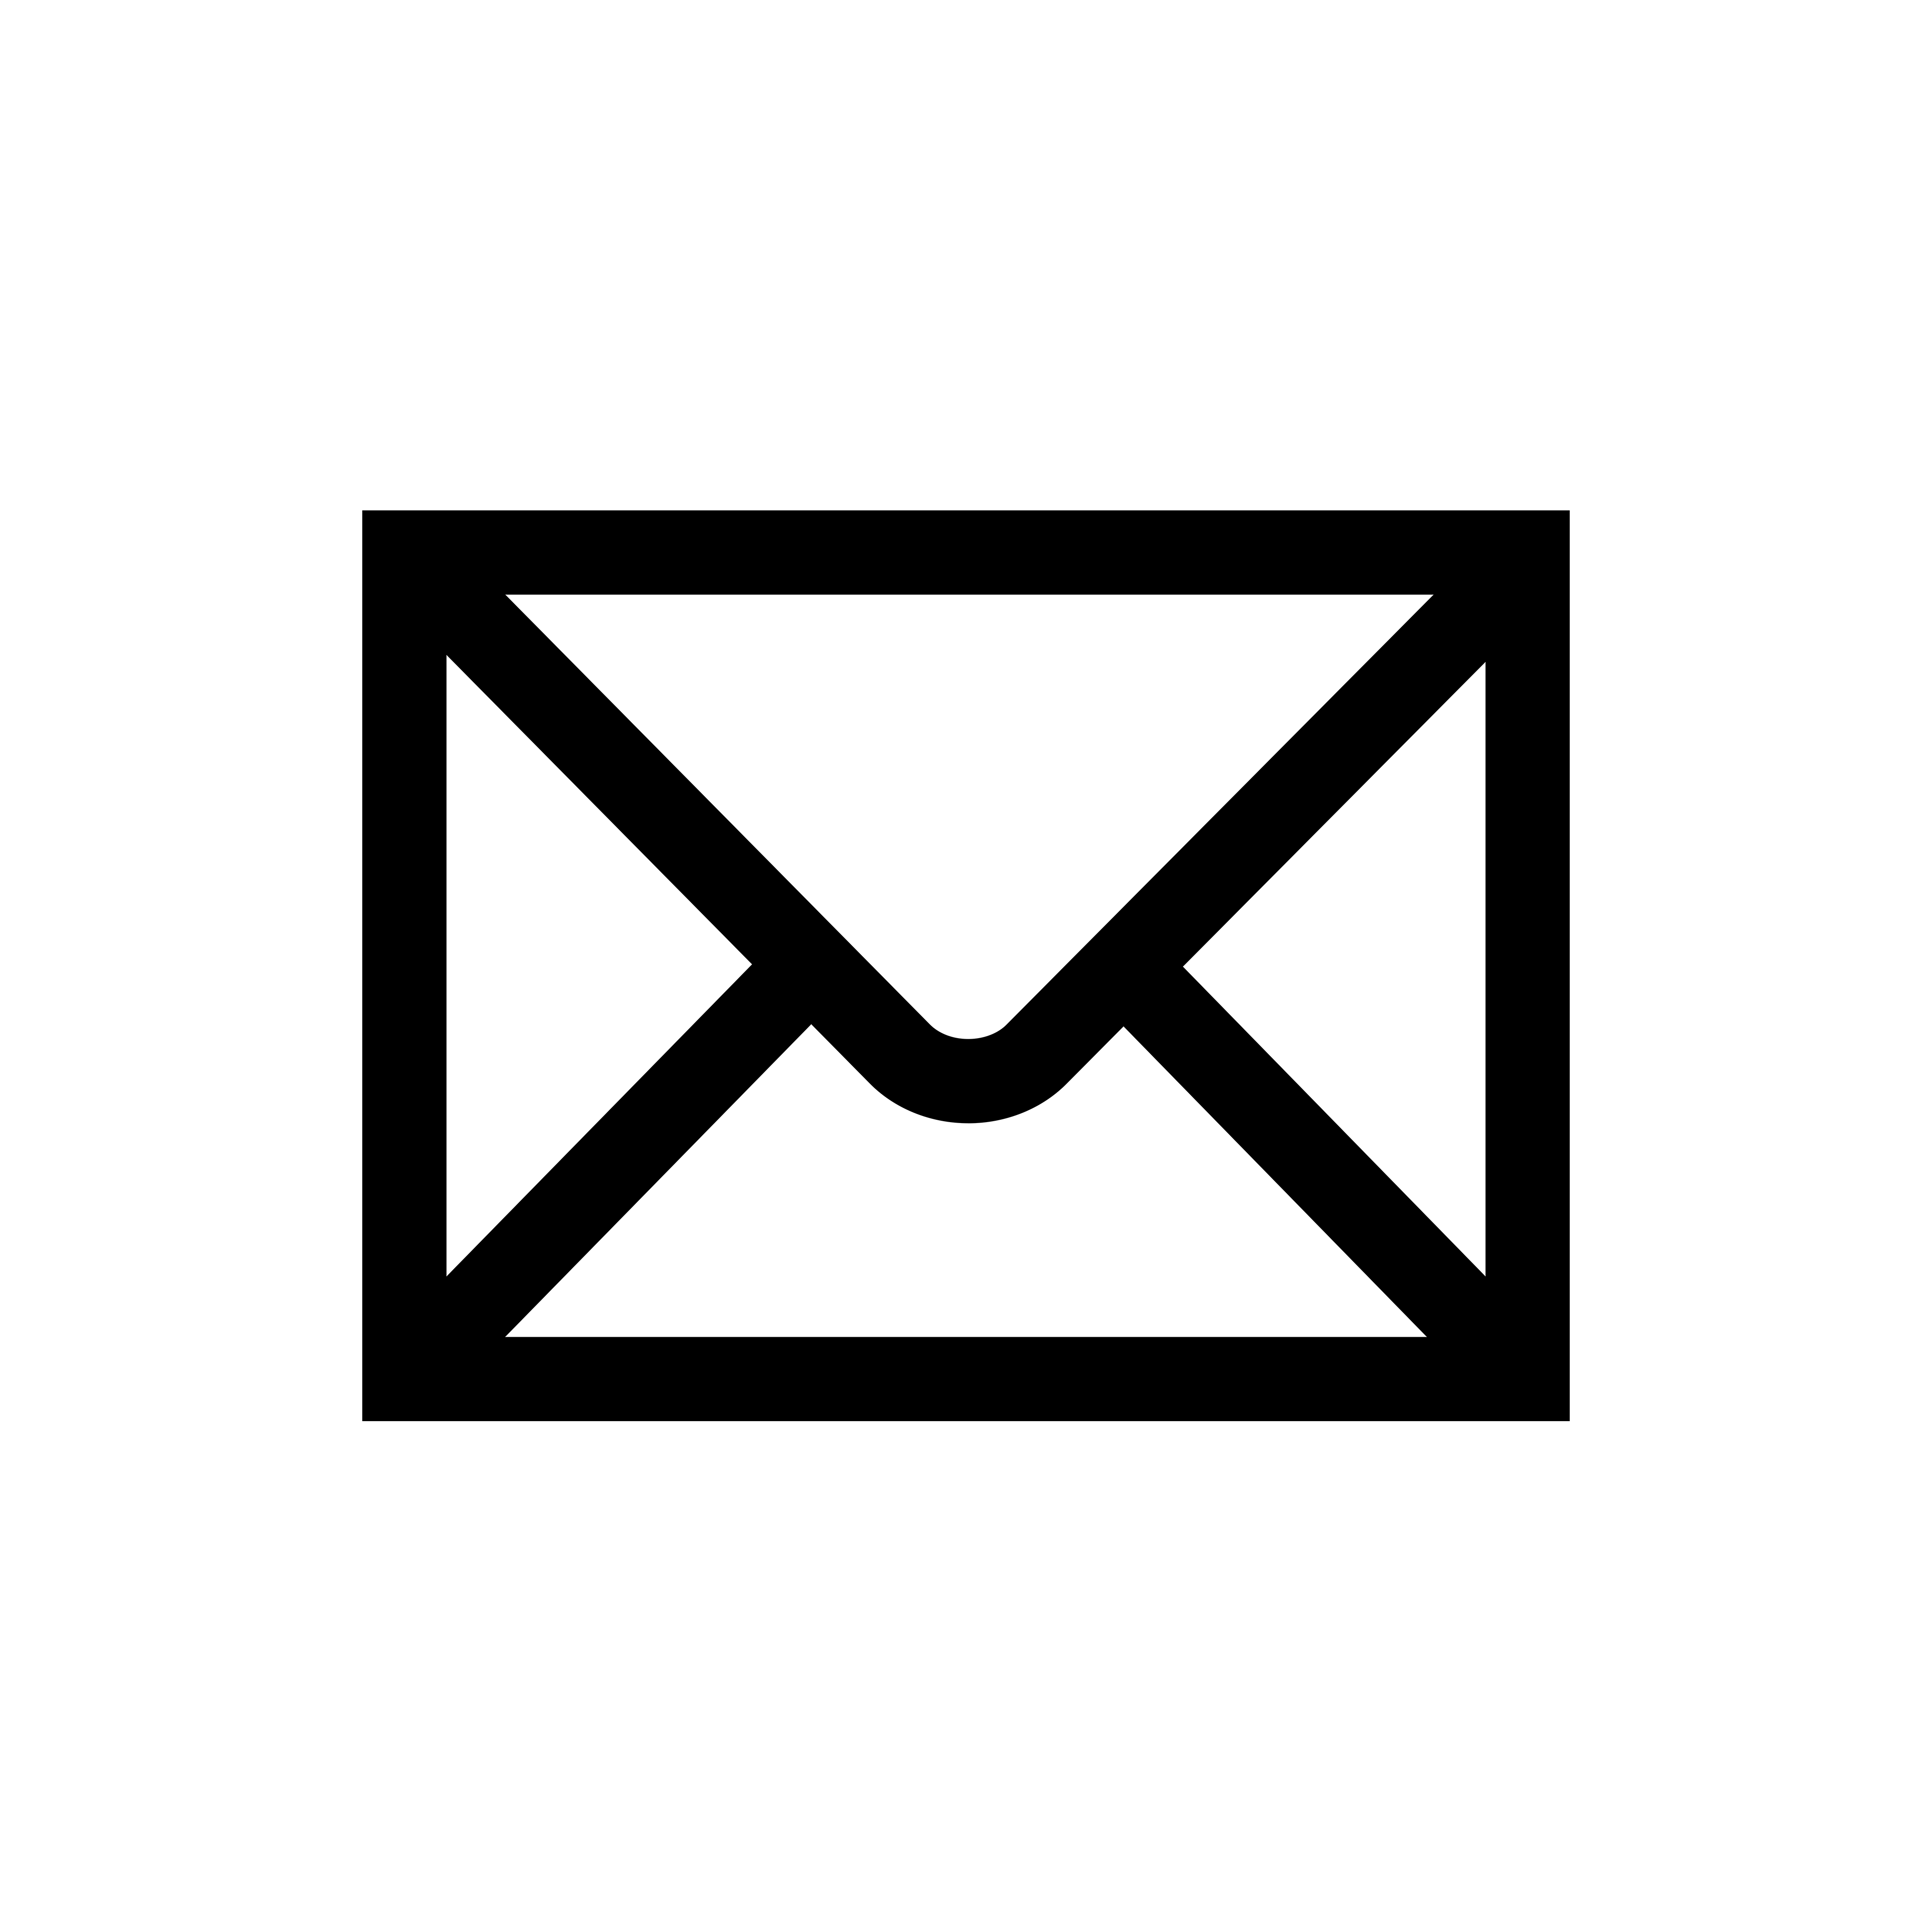
\includegraphics[width=0.018\textwidth]{images/email.png} \raisebox{0.006\textwidth}{\TheEmail}\\[\baselineskip]
}
}

% title goes here
\TheTitle{This is an Extremely Long Title \\ that will Span Several Lines on the Poster}

% author(s) go(es) here
\TheAuthors{\underline{Author One}\textsuperscript{1}, Author Two\textsuperscript{2} and Author Three\textsuperscript{1}\\
  {\footnotesize \textsuperscript{1}KU Leuven, \textsuperscript{2}Some Minor University}}
  
% corresponding author email goes here
\TheEmail{author.one@kuleuven.be}

\begin{document}

% poster environment
% options are
% \begin{poster}{number of columns}{title}{author}{institute/university logo(s)}{company/funding agency logo(s)}{true/false for dutch}
\begin{poster}{3}{\title}{\author}
{% Logo's of associated institutes/universities etc.
  
\includegraphics[height=.8\footerheight]{figures/logo_ecoleponts.pdf}\hspace{2em}%
  
\includegraphics[height=.8\footerheight]{figures/logo_stanford.jpg}%
}{% Logo's of companies/funding etc.
  
\includegraphics[height=.8\footerheight]{figures/logo_euforia.png}\hspace{1em}% 
}{
% "true" if this is a dutch poster
}

% A poster contains boxes. You can choose between a \heavybox or a \lightbox.
% The boxes are fully customizable if you use the lower level posterbox environment, see below.
\heavybox{In a Nutshell}{
	name=in a nutshell,
	column=0,
	row=0
}{
	\begin{description} % a description contains a list of keywords with explanation
		\item[Goal] Make the best poster template ever created for the Department of Computer Science of KU Leuven
		\item[Model] A mathematical model of a poster
		\item[Method] Awesome \LaTeX\ skills
		\item[Result] This beautiful poster
		\item[Bonus] Present your research in a unified way in agreement with the department's standard
	\end{description}
}

\lightbox{Mathematical Model}{
	name=mathematical model,
	column=0,
	below=in a nutshell
}{
	\begin{noindentitemize} % default itemize environment
		\item We can specify a mathematical model using the usual \texttt{align} environment
		\item For example, the Maxwell equations are
		\begin{align}
    		\Rot\vec{E} &=-\frac{1}{c}\parder{\vec{B}}{t},\\
    		\Div\vec{B} &=0,\\
    		\Rot\vec{B} &=\frac{1}{c}\parder{\vec{E}}{t}+\frac{4\pi}{c}\,\vec{j},\\
    		\Div\vec{E} &=4\pi\rho_{\varepsilon}
		\end{align}
		\item For good practice, don't terminate your sentence with a . (``dot'') on a scientific poster
	\end{noindentitemize}
}

\heavybox{A Small Sidenote}{
	name=a small sidenote,
	column=0,
	above=bottom
}{
	\begin{description}
		\item[Notice] At vero eos et accusamus et iusto odio dignissimos ducimus qui blanditiis praesentium voluptatum deleniti atque corrupti quos dolores et quas molestias excepturi sint occaecati cupiditate non provident
		\item[Solution] Et harum quidem rerum facilis est et expedita distinctio nam libero tempore, cum soluta nobis est eligendi optio cumque nihil impedit:
		\begin{align}
			\int_0^\infty e^{-x^2} dx=\frac{\sqrt{\pi}}{2}
		\end{align}
		Nullam quis ante etiam sit amet orci eget eros faucibus tincidunt duis leo
	\end{description}
}

\lightbox{Yet Another \texttt{posterbox}}{
	name=yet another poster box,
	column=0,
	below=mathematical model,
	above=a small sidenote
}{
	\begin{noindentitemize}
		\item You can choose between a \texttt{\textbackslash heavybox} or a \texttt{\textbackslash lightbox} (this one), or use the lower level \texttt{posterbox}-environment
		\item Several options for \texttt{\textbackslash textborder} are available:\\ 
		\texttt{none}\\
		\texttt{bars}\\
		\texttt{rectangle}\\
		\texttt{onlyleft}\\
		\texttt{onlytop}\\
		\texttt{hookbox}\\
		\texttt{hook}
		\item Lorem ipsum dolor sit amet, consectetuer adipiscing elit ut purus elit, vestibulum ut, placerat ac, adipiscing vitae, felis
		\begin{align}
    		e=mc^2
		\end{align}
		\item Curabitur dictum gravida mauris nam arcu libero, nonummy eget, consectetuer id, vulputate a, magna donec 
		\item Pellentesque habitant morbi tristique senectus et netus
	\end{noindentitemize}
}

\lightbox{Some Figures}{
	name=some figures,
	column=1,
	row=0
}{
	\centering
	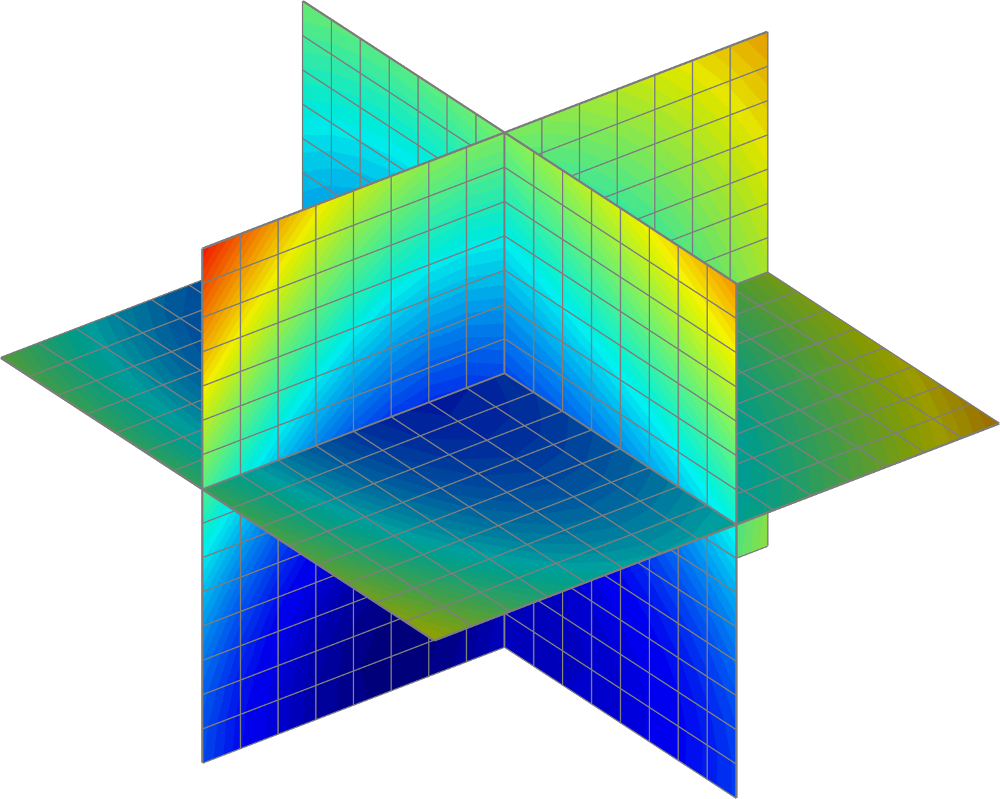
\includegraphics[width=0.8\textwidth]{figures/sample_field_F1.png}\\
	$\Phi = \{1,1,2.5\}$\vspace{1em}\\
	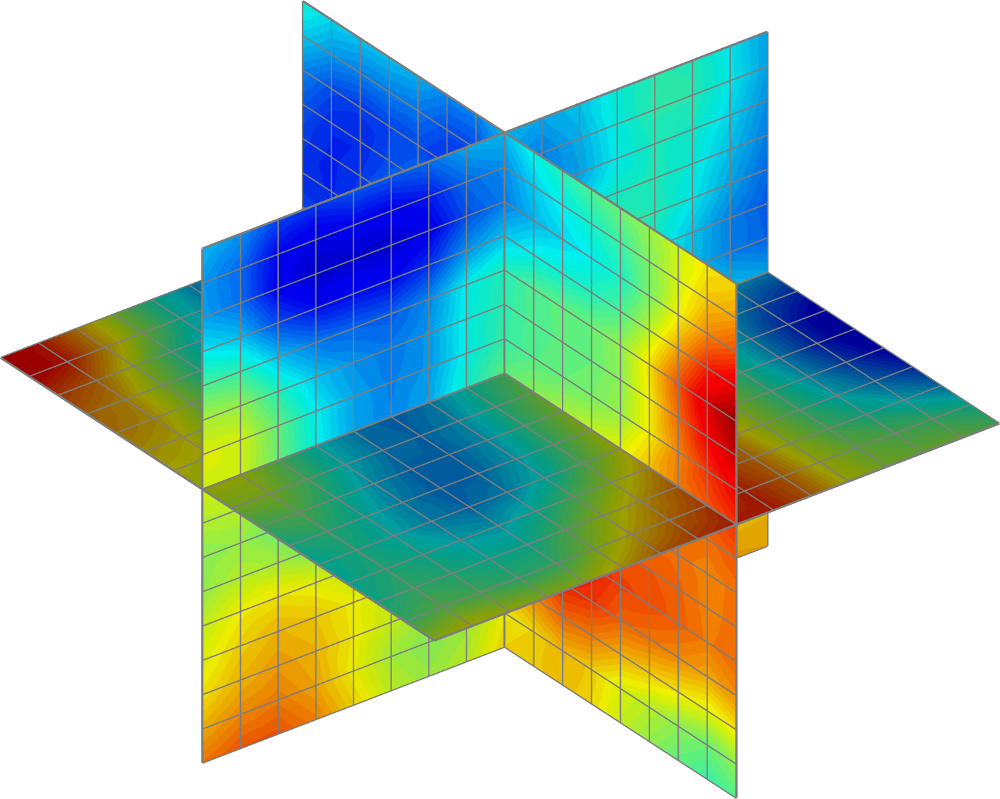
\includegraphics[width=0.8\textwidth]{figures/sample_field_F2.png}\\
	$\Phi = \{0.3,1,1\}$\vspace{1em}\\
	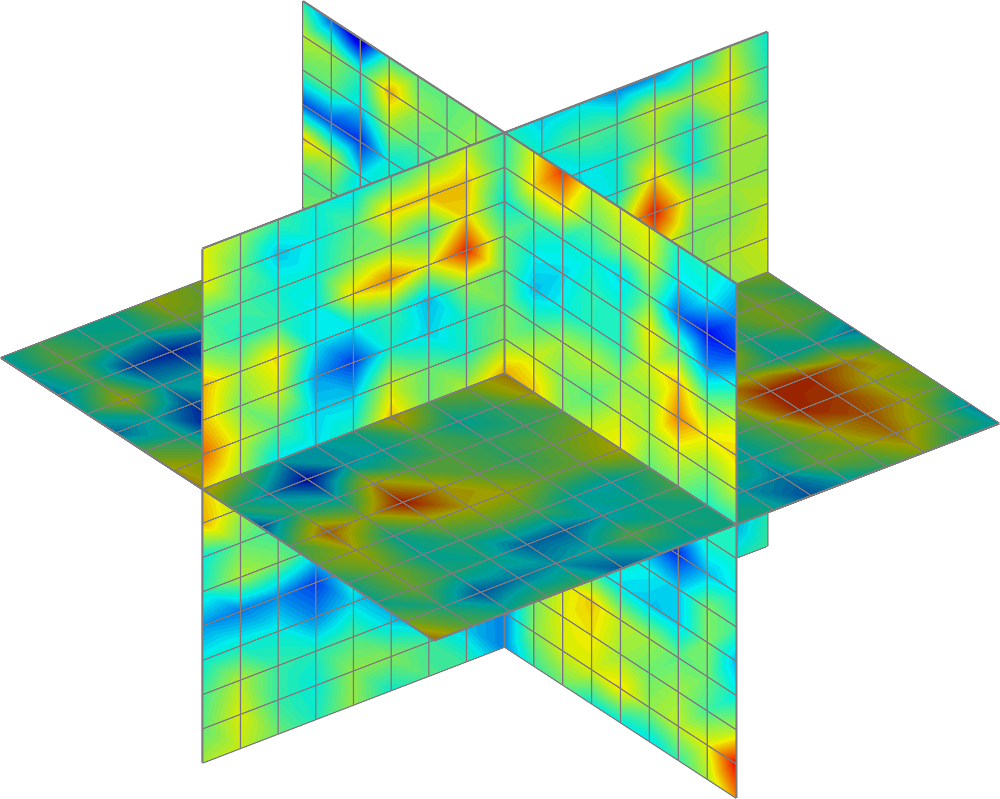
\includegraphics[width=0.8\textwidth]{figures/sample_field_F3.png}\\
	$\Phi = \{0.1,1,0.5\}$\\
}

\lightbox{The Method}{
	name=the method,
	column=1,
	below=some figures,
	above=bottom
}{
	\begin{noindentitemize}
		\item Maecenas vestibulum mollis diam pellentesque ut neque pellentesque habitant morbi tristique senectus et netus
		\item In dui magna, posuere eget, vestibulum et, tempor auctor, justo in ac felis quis tortor malesuada pretium pellentesque auctor neque nec urna proin sapien ipsum
		\begin{align}
		F(x,y)=0 \quad \mbox{and} \quad
		\begin{pmatrix}
  			F''_{xx} & F''_{xy} &  F'_x \\
  			F''_{yx} & F''_{yy} &  F'_y \\
  			F'_x     & F'_y     & 0 
  			\end{pmatrix} = 0
		\end{align}
		\item Phasellus magna in hac habitasse platea dictumst
		\begin{align}
			\begin{split}
				a_n=\frac{1}{\pi}\int\limits_{-\pi}^{\pi}f(x)\cos nx\,\mathrm{d}x\\
					=\frac{1}{\pi}\int\limits_{-\pi}^{\pi}x^2\cos nx\,\mathrm{d}x
			\end{split}\\
			\begin{split}
				b_n=\frac{1}{\pi}\int\limits_{-\pi}^{\pi}f(x)\sin nx\,\mathrm{d}x\\
					=\frac{1}{\pi}\int\limits_{-\pi}^{\pi}x^2\sin nx\,\mathrm{d}x
			\end{split}
		\end{align}
	\end{noindentitemize}
}

\heavybox{Simulation Details}{
	name=simulation details,
	column=2,
	row=0
}{
	\begin{noindentitemize}
		\item This is a list of countries
	\end{noindentitemize}
	\begin{center}
		\begin{tabular}{ lcc} \toprule
 			country 									& extension 	& code \\ \midrule
			Andorra 									&	.ad					& AD	\\
			United Arab Emirates			&	.ae					& AE	\\	
			Afghanistan								&	.af					& AF	\\
			Antigua and Barbuda			&	.ag					& AG	\\
			Anguilla									&	.ai					& AI	\\
			Albania										&	.al					& AL \\
			Armenia									&	.am					& AM	 \\
			Angola										&	.ao					& AO	 \\
			Antarctica									&	.aq					& AQ \\
			Argentina									&	.ar					& AR	\\
			American Samoa					&	.as					& AS	\\
			Austria										&	.at					& AT	\\
			Australia									&	.au					& AU	\\
			Aruba										&	.aw					& AW \\
			Aaland Islands						&	.ax					& AX	\\
			Azerbaijan								&	.az					& AZ	\\
			Bosnia and Herzegovina	&	.ba					& BA	\\
			Barbados									&	.bb					& BB	\\
			Bangladesh								&	.bd					& BD \\
			Belgium										&	.be					& BE \\ \bottomrule
		\end{tabular}
	\end{center}
}

% adding references, now using the "posterbox" environment
\begin{posterbox}
	[
		name=references,
		column=2,
		above=bottom,
		borderColor=KULeuvenDeptCS,
		textborder=onlyleft,
		boxshade=none,
		headerColorOne=KULeuvenDeptCS,
		headerBorderColor=KULeuvenDeptCS,
		boxheaderheight=2em,
		headerFontColor=white
	]
	{References}
	\begin{enumerate}[label={[\arabic*]}]
		\item Aurentz, Jared L., Mach, T. and Vandebril, R., \emph{Fast and Backward Stable Computation of Roots of Polynomials}, SIAM Journal on Matrix Analysis and Applications, 36(3):942--973, 2015.
		\item Cools, R. and Rabinowitz, P., \emph{Monomial Cubature Rules since ``Stroud'': a Compilation}, Journal of Computational and Applied Mathematics, 48(3):309--326, 1993.
		\item Einstein, A., \emph{Zur Elektrodynamik bewegter K{\"o}rper}. (German) [\emph{On the Electrodynamics of Moving Bodies}], Annalen der Physik, 322(10):891--921, 1905.
	\end{enumerate}
\end{posterbox}

\lightbox{Results}{
	name=results,
	column=2,
	below=simulation details
}{
	The Hertzsprung--Russell diagram:
	\begin{center}
	\includetikz{hertzsprung-russell} % easy tikz macro
	\end{center}
}

\heavybox{Conclusions}{
	name=conclusions,
	column=2,
	above=references,
	below=results
}{
	\begin{description}
		\item[Summary] We have shown a poster template for the Department of Computer Science of KU Leuven
		\item[Contribution] The Department of Computer Science is the best!
	\end{description}
}

\end{poster}

\end{document}